\documentclass[11pt]{article}
\usepackage[final]{acl}
\usepackage{times}
\usepackage{latexsym}
\usepackage[T1]{fontenc}
\usepackage[utf8]{inputenc}
\usepackage{microtype}
\usepackage{graphicx}
\usepackage{amsmath}
\usepackage{amssymb}
\usepackage{booktabs}
\usepackage{array}
\usepackage{tikz}
\usetikzlibrary{positioning,arrows.meta}
\urlstyle{same}

% ---- replace with your public repository URL before submission ----
\newcommand{\repourl}{https://github.com/YOUR-USERNAME/COMP8240-FakingFakeNews-Replication}

\title{Final Report: Reproducing and Extending Propaganda-Loaded Training Data Generation for Fake News Detection}

\author{
Atharva Chitgopekar \\
Master of Data Science, Macquarie University \\
OneID: 48934941 \\
atharvaanand.chitgopekar@students.mq.edu.au
}

\begin{document}
\maketitle

\begin{abstract}
We replicate the RoBERTa-large detector of \citet{huang-etal-2023-faking}, which is trained on PropaNews, a corpus of propaganda-loaded synthetic fake news, and test how well it generalises to new data. Using the authors' code and data on a single Colab T4 GPU, our replication reaches an AUC of 57.8 on PolitiFact and 43.3 on Snopes, against the paper's 65.3 and 53.0. A per-epoch analysis traces the gap to a training collapse that coincides with the peak of the learning-rate schedule. We then evaluate the replicated detector on two existing datasets the method has not been applied to, LIAR and WELFake, and on WikiPropaNews, a new 594-article test set that we construct from openly licensed Wikinews articles (2020--2026) following the PropaNews recipe: one salient sentence per article is replaced with an NLI-verified false claim, optionally with loaded language or an appeal to authority. The detector transfers to LIAR and WELFake about as well as to PolitiFact (AUC 0.56--0.58), but cannot separate WikiPropaNews articles from their real counterparts (AUC 0.52). Within matched article pairs, however, it significantly lowers its real-news probability when propaganda techniques are present ($p<0.01$), but not when only a false claim is inserted. This suggests that what the detector has learned is propagandistic style rather than falsity.
\end{abstract}

\section{Introduction}

Detectors of fake news are usually trained on machine-generated text, but must operate on disinformation written by people with persuasive intent. \citet{huang-etal-2023-faking} narrow this gap by generating training articles that mimic human propaganda, and report that detectors trained on their PropaNews corpus transfer better to human-written fake news. This report documents a reproducibility study of that claim, organised around three research questions:

\paragraph{RQ1.} Can the paper's reported transfer results be reproduced with the released code and data? (Section~\ref{sec:replication})

\paragraph{RQ2.} Does the trained detector generalise to existing datasets the paper did not use, namely LIAR and WELFake? (Sections~\ref{sec:newdata} and~\ref{sec:results})

\paragraph{RQ3.} Does it generalise to a new, recent test set built with the PropaNews recipe, and to which propaganda techniques does it respond? (Sections~\ref{sec:newdata} and~\ref{sec:results})

\vspace{4pt}
Section~\ref{sec:ethics} discusses ethics, and Section~\ref{sec:conclusion} answers the three questions. Our contributions are: (i) a documented replication, including two code--paper discrepancies and a per-epoch diagnosis of training collapse; (ii) a corrected evaluation on LIAR, after we found that our earlier label mapping inverted the repository's label convention; (iii) WikiPropaNews, a balanced, openly licensed, NLI-filtered test set validated by an LLM judge and a human annotator; and (iv) a paired, within-article analysis that isolates the effect of propaganda techniques on the detector's scores. All of our scripts, generated data and analysis outputs are publicly available.\footnote{Project repository: \url{\repourl}}

\section{The Original Paper and Justification}
\label{sec:paper}

\citet{huang-etal-2023-faking}\footnote{Paper: \url{https://aclanthology.org/2023.acl-long.815/}} generate fake news in two stages. In the first stage, an extractive summariser identifies the most salient sentence of an authentic article, and BART replaces it with plausible but false content. The generator is trained with self-critical sequence training \citep{rennie2017selfcritical}, using a reward that penalises outputs entailed by the original sentence according to an MNLI-trained RoBERTa model \citep{williams2018mnli}. In the second stage, two propaganda techniques \citep{dasanmartino2019finegrained} may be added. Appeal to authority inserts a quotation from a real authority figure, drawn from Wikidata, that supports the false claim. Loaded language inserts emotionally charged modifiers, using a BART model trained on annotated loaded-language spans. Crowdworkers then verify that each generated sentence is indeed inaccurate.

The result, PropaNews, contains 2,256 articles built from TIMELINE17 news \citep{tran2013timeline}. It is balanced between real and fake articles; among the fakes, 30\% use appeal to authority, 30\% use loaded language, and 40\% contain only false information.

\paragraph{Evaluation framework.} Detectors are trained on PropaNews, selected on its development split, and tested on human-written articles from Snopes \citep{nguyen2020fang} and PolitiFact \citep{shu2018fakenewsnet}. The main results table reports ROC AUC as the mean and standard deviation of four runs, with significance tested by a paired bootstrap. The abstract, by contrast, states the headline gain over baseline training corpora as 3.62--7.69 F1 points. For RoBERTa-large trained on PropaNews, the paper reports AUC $65.34\pm4.5$ on PolitiFact and $53.03\pm3.7$ on Snopes. The best competing corpus, Grover-Gen, reaches 57.65 and 48.42.

\paragraph{Justification.} The paper appeared in the main track of ACL 2023, which is ranked A* in CORE and is among the highest-ranked venues in Google Scholar's Computational Linguistics category. Its authors are from UIUC, Columbia, MBZUAI, the University of Washington and AI2, and at the time of our proposal it had over 100 Google Scholar citations. It is also highly reproducible: the code and all evaluation data are public. It addresses a socially important problem, and its central claim, that training data which mimic human propaganda transfer better, is falsifiable on new data.

\section{Original Datasets}
\label{sec:origdata}

The authors' repository\footnote{Code and data: \url{https://github.com/khuangaf/FakingFakeNews}} contains five JSON-lines files (Table~\ref{tab:origdata}). Each line is one article, stored as a text field holding the pre-tokenised title and body concatenated, and a Boolean label. The PropaNews files also carry a file path whose suffix encodes the type of fake: ``sent-fake'' for plain disinformation, ``ll\_filled'' for loaded language and ``app-auth-final'' for appeal to authority. We counted 440, 388 and 300 of these across all splits. The Snopes and PolitiFact counts match the paper's appendix exactly. Table~\ref{tab:snippet} shows two truncated records.

Inspecting the files exposed a detail that the paper does not state and that our proposal had described wrongly: a label of true denotes real news. The detector's sigmoid output is therefore $P(\text{real})$, and the repository's F1 treats real as the positive class. We follow this convention throughout.

\begin{table}[t]
\centering\small
\begin{tabular}{lrrrr}
\toprule
File & $n$ & real & fake & words$^\dagger$ \\
\midrule
PropaNews train & 1,256 & 645 & 611 & 815 \\
PropaNews dev & 500 & 240 & 260 & 782 \\
PropaNews test & 500 & 243 & 257 & 851 \\
Snopes & 710 & 430 & 280 & 425 \\
PolitiFact & 886 & 517 & 369 & 303 \\
\bottomrule
\end{tabular}
\caption{Datasets distributed with the original code. $^\dagger$Median whitespace tokens.}
\label{tab:origdata}
\end{table}

\begin{table}[t]
\centering\small
\begin{tabular}{@{}>{\raggedright\arraybackslash}p{0.2\columnwidth}>{\raggedright\arraybackslash}p{0.74\columnwidth}@{}}
\toprule
Field & Value \\
\midrule
\multicolumn{2}{@{}l}{PropaNews training record (loaded-language fake)} \\
text & LONDON | Thu Oct 7, 2010 7:41 am EDT LONDON (Reuters) - U.S. oil explorers are talking about forming a new insurance fund that would cover the costs of any future oil spill \ldots \\
label & false (fake) \\
path & \ldots/bpoil\_reuters\_\_2010-10-07\_\_1470.rsd.txt.ll\_filled \\
\midrule
\multicolumn{2}{@{}l}{Snopes test record} \\
text & Hostages held in Sydney cafe, Islamic flag seen in window: local TV. SYDNEY (Reuters) - Hostages were being held inside a central Sydney cafe \ldots \\
label & true (real) \\
\bottomrule
\end{tabular}
\caption{Snippet of the original data: one record from each kind of file, truncated.}
\label{tab:snippet}
\end{table}

\section{Replication of the Original Work}
\label{sec:replication}

\begin{table}[t]
\centering\small
\setlength{\tabcolsep}{3pt}
\footnotesize\begin{tabular}{lll}
\toprule
 & Paper & Ours \\
\midrule
Hardware & V100 & T4 (Colab) \\
Software & PyTorch 1.10, & PyTorch 2.14, \\
 & Transformers 4.3 & Transformers 5.22 \\
Optimiser & AdamW & PyTorch AdamW$^\ddagger$ \\
Batch $\times$ accum. & $2\times8$ & $2\times8$ \\
LR enc./head & 5e-5 / 1e-3 & 5e-5 / 1e-3 \\
Epochs & $\le$20 (code: 30) & 10 \\
Selection & dev accuracy & dev AUC (code) \\
Runs & 4 (mean) & 1 (seed 42) \\
Train time & 2--3 h & 73 min \\
\bottomrule
\end{tabular}
\caption{Training set-up of the paper (its appendix and code) and of our replication. $^\ddagger$Replaces the AdamW class that has been removed from the Transformers library.}
\label{tab:env}
\end{table}

\paragraph{Environment and procedure.} Table~\ref{tab:env} summarises the set-up. We used Google Colab with a Tesla T4 (16\,GB), Python 3.13, PyTorch 2.14, Transformers 5.22 and scikit-learn 1.6. The paper used a V100 with PyTorch 1.10 and Transformers 4.3. Getting the code to run required two changes. First, the Transformers library no longer provides AdamW, so we import PyTorch's AdamW instead; our repository applies this one-line patch with a setup script. Second, the authors' trained checkpoint is no longer available from its Google Drive link, so we had to train from scratch.

We kept every hyperparameter at the repository's defaults: batch size 2 with 8 accumulation steps, learning rates of $5\times10^{-5}$ for the encoder and $10^{-3}$ for the head, a maximum length of 512, 5 warm-up epochs and seed 42. The only change was the number of epochs. We trained for 10 instead of the default 30: one epoch takes 7.3 minutes, and an earlier 30-epoch attempt was lost when Colab's GPU quota disconnected the session. The training script reports results on Snopes, and the test script reports PolitiFact because the filename is hard-coded in it.

\paragraph{Code--paper discrepancies.} The paper states that detectors were trained ``for at most 20 epochs'' with the best model ``determined by the accuracy on the development set''. The code instead defaults to 30 epochs and, although its log line says ``dev accuracy'', it selects checkpoints by dev AUC: the variable holding accuracy is overwritten with AUC before the comparison.

\begin{table}[t]
\centering\small
\setlength{\tabcolsep}{4pt}
\begin{tabular}{lcc}
\toprule
 & Paper (4 runs) & Ours (1 run, 95\% CI) \\
\midrule
PolitiFact AUC & $65.34\pm4.5$ & 57.76 [53.7, 61.5] \\
Snopes AUC & $53.03\pm3.7$ & 43.32 [38.9, 47.9] \\
\midrule
\multicolumn{3}{l}{Ours, threshold 0.5: PolitiFact acc.\ 54.9, macro-F1 54.6;} \\
\multicolumn{3}{l}{\quad Snopes acc.\ 44.5, macro-F1 42.9.} \\
\bottomrule
\end{tabular}
\caption{Replicated RoBERTa-large trained on PropaNews. Paper values are mean $\pm$ s.d.; ours carry 1,000-sample bootstrap CIs.}
\label{tab:replication}
\end{table}

\begin{figure}[t]
\centering
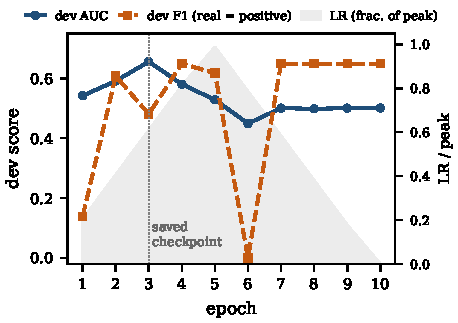
\includegraphics[width=\columnwidth]{fig_training.pdf}
\caption{Development-set dynamics of our 10-epoch run. The grey area shows the learning-rate schedule (5-epoch linear warm-up, then linear decay). After the learning rate peaks, the model collapses to a constant output: dev AUC is exactly 0.5 and dev F1 alternates between 0 (always fake) and 0.649 (always real).}
\label{fig:training}
\end{figure}

\paragraph{Results.} Table~\ref{tab:replication} compares our results with the paper's. On PolitiFact our AUC is 7.6 points lower, about 1.7 of the paper's standard deviations, and our 95\% CI excludes the paper's mean. On Snopes it is 9.7 points lower, and our whole CI lies below chance. In neither case do we reproduce the reported advantage over the strongest baseline. As a consistency check on our own tooling, the Snopes AUC computed by our evaluation script (0.4332) matches the value printed by the original training script (0.4330).

\paragraph{Why the results differ.} The training log (Figure~\ref{fig:training}; Appendix~\ref{app:log}) gives the most direct explanation. Dev AUC rises to 0.655 at epoch 3, which becomes the saved checkpoint. From epoch 6 onwards the model collapses to a constant prediction: dev AUC is exactly 0.500, and F1 jumps between 0 and 0.649 depending on which class the constant output falls on. The training loss barely moves, from 465 to 436.

The collapse coincides with the end of warm-up, when the encoder reaches its peak learning rate while the randomly initialised head is trained at $10^{-3}$. This pattern matches the documented instability of fine-tuning large pre-trained encoders on small datasets \citep{mosbach2021stability}, and PropaNews has only 1,256 training examples. Because the paper's 30-epoch default has the same 5-epoch warm-up, the longer schedule alone would not have avoided the peak. The paper's four-run average, and its large standard deviation, suggest that run-to-run variance is substantial even under the original setup.

Several further factors plausibly contribute:
(i) Our checkpoint was saved mid-warm-up and is under-trained. On WikiPropaNews its $P(\text{real})$ never exceeds 0.55 (Figure~\ref{fig:hist}).
(ii) We report a single seed, where the paper averages four.
(iii) Checkpoints are selected on in-domain PropaNews dev AUC, which need not track transfer to human-written news.
(iv) Our library stack is four years newer than the paper's.

Earlier feasibility runs reported in our proposal (a 1-epoch run with F1$=$0, and a 2-epoch run without warm-up) showed the same tendency towards degenerate outputs. We therefore regard the replication as partial: the pipeline runs end to end and produces meaningful above-chance transfer to PolitiFact, but the reported effect sizes were not reproduced. All later results describe the generalisation of this particular checkpoint, which is a lower bound on what the original method achieves.

\section{Construction of New Data}
\label{sec:newdata}

\subsection{Existing Datasets New to the Method}

\paragraph{LIAR.} LIAR \citep{wang2017liar} contains short PolitiFact statements on a six-point truth scale; we use its test split of 1,283 statements, averaging 18 words each. We made a binary version, mapping true, mostly-true and half-true to real (727 statements) and barely-true, false and pants-fire to fake (556). We also made a strict version that drops the ambiguous half-true class (1,016 statements).

While preparing the final evaluation, we found that our update-stage mapping had coded real news as 0, the opposite of the repository's convention. The update-stage AUC of 0.438 was therefore the complement of the true value, since inverting labels turns AUC into $1-\text{AUC}$. Re-running with correct labels gives 0.564, matching the predicted $1-0.438=0.562$.

\paragraph{WELFake.} WELFake \citep{verma2021welfake} merges Kaggle, McIntire, Reuters and BuzzFeed articles; its length matches PropaNews, so it tests transfer on full articles. Rather than assume what the labels mean, we checked them against the data. Reuters wire copy is real news, and 99.9\% of the 17,478 articles containing ``(Reuters)'' carry label 0, so we treat 0 as real. This is the opposite of the convention often assumed for this dataset.

After de-duplicating and filtering to articles of 100--1,500 words, we drew a balanced sample of 1,000 articles (seed 42). We also removed the ``(Reuters)'' dateline, which would otherwise reveal the label directly.

\subsection{WikiPropaNews: A Newly Constructed Test Set}

\paragraph{Design and pilot.} Our proposal planned to rewrite recent real articles in a propaganda-loaded style using an off-the-shelf LLM. The update-stage pilot did this for 5 pairs and revealed two weaknesses. Its real side consisted of summaries we had written ourselves, and its fakes kept every fact, so they were sensationalised true news rather than disinformation. The final design therefore follows the PropaNews recipe more closely (Figure~\ref{fig:pipeline}). It uses genuine published articles, alters exactly one salient sentence to make it false, and optionally adds a propaganda technique. Every fake is paired with its unaltered original.

\begin{figure}[t]
\centering
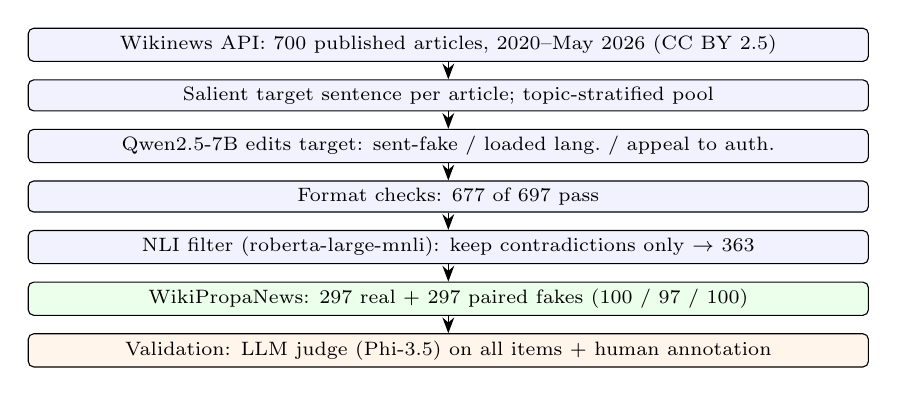
\begin{tikzpicture}[node distance=2.2mm, every node/.style={font=\scriptsize, align=center},
  box/.style={draw, rounded corners=2pt, fill=blue!5, minimum width=0.88\columnwidth, inner sep=2.5pt},
  arr/.style={-{Stealth[length=2mm]}}]
\node[box] (a) {Wikinews API: 700 published articles, 2020--May 2026 (CC BY 2.5)};
\node[box, below=of a] (b) {Salient target sentence per article; topic-stratified pool};
\node[box, below=of b] (c) {Qwen2.5-7B edits target: sent-fake / loaded lang.\ / appeal to auth.};
\node[box, below=of c] (d) {Format checks: 677 of 697 pass};
\node[box, below=of d] (e) {NLI filter (roberta-large-mnli): keep contradictions only $\rightarrow$ 363};
\node[box, below=of e, fill=green!8] (f) {WikiPropaNews: 297 real + 297 paired fakes (100 / 97 / 100)};
\node[box, below=of f, fill=orange!8] (g) {Validation: LLM judge (Phi-3.5) on all items + human annotation};
\foreach \x/\y in {a/b,b/c,c/d,d/e,e/f,f/g} \draw[arr] (\x) -- (\y);
\end{tikzpicture}
\caption{The WikiPropaNews construction pipeline.}
\label{fig:pipeline}
\end{figure}

\paragraph{Source and collection.} Real articles come from English Wikinews \citep{wikinews}. Its articles are reviewed before publication, dated and openly licensed (CC BY 2.5), so the dataset can be redistributed publicly with attribution. The archive has also been read-only since the project closed in May 2026, so our collection is reproducible.

Wikinews' category timestamps do not reflect publication dates, so we scanned published pages newest first and took each article's date from its own dateline, falling back to its first revision when no dateline was present. We kept articles of 150--1,500 words and excluded news-brief compilations, interviews and opinion pieces. This yielded 700 articles from 2020 onwards. The window post-dates both PropaNews' 2009--2013 source news and RoBERTa's 2019 pre-training corpus \citep{liu2019roberta}.

\paragraph{Target sentences and generation.} The paper selects target sentences with an extractive summariser. As a lightweight stand-in, we score sentences 2--11 of each article by checkable-fact density: twice the number of numeric tokens plus the number of capitalised tokens. We require each candidate to be 12--50 words long, contain no direct quotation and occur exactly once in the article, and take the highest-scoring sentence. A topic-stratified round-robin then draws a pool of 540 articles, with fake types assigned in rotation.

Generation uses Qwen2.5-7B-Instruct \citep{qwen2024qwen25}, quantised to 4-bit NF4 \citep{dettmers2023qlora}, with temperature 0.7 and top-$p$ 0.9. One prompt per fake type mirrors PropaNews' three types (Appendix~\ref{app:prompts}). As an ethical safeguard, generated quotations must be attributed to unnamed authorities, never to real named people. Outputs must also pass format checks: a changed sentence, a length ratio between 0.5 and 2, no refusal, and an actual quotation for appeal-to-authority fakes.

\paragraph{NLI filtering.} Following the paper, we use roberta-large-mnli and keep a fake only if the original sentence contradicts the generated one (Table~\ref{tab:nli}). The pass rates expose a clear trade-off. Plain falsification succeeded 88\% of the time. Adding a quotation lowered this to 66\%, and asking for loaded language lowered it to 29\%: the model mostly restyled the sentence and left its facts intact, as in our pilot. We therefore ran an extra 157 loaded-language generations on the unused articles. The paper avoids this problem by generating the false claim first and adding propaganda as a separate step; prompting for both at once does not.

\begin{table}[t]
\centering\small
\setlength{\tabcolsep}{4pt}
\begin{tabular}{lrrrr}
\toprule
Fake type & $n$ & contrad. & neutral & entail. \\
\midrule
sent-fake & 180 & 88.3\% & 3.9\% & 7.8\% \\
appeal-to-authority & 162 & 66.0\% & 24.7\% & 9.3\% \\
loaded-language & 335 & 29.0\% & 69.6\% & 1.5\% \\
\bottomrule
\end{tabular}
\caption{NLI labels (original $\rightarrow$ generated sentence) for all 677 format-valid generations.}
\label{tab:nli}
\end{table}

\begin{table}[t]
\centering\small
\setlength{\tabcolsep}{2pt}
\footnotesize\begin{tabular}{lrrrrl}
\toprule
Dataset & $n$ & real & fake & words$^\dagger$ & Source \\
\midrule
LIAR & 1,283 & 727 & 556 & 18 & PolitiFact \\
LIAR-strict & 1,016 & 460 & 556 & 18 & PolitiFact \\
WELFake & 1,000 & 500 & 500 & 100--1.5k & 4 outlets \\
WikiPropaNews & 594 & 297 & 297 & 344 & Wikinews \\
\bottomrule
\end{tabular}
\caption{New test data. $^\dagger$Mean words (for WELFake, the length filter applied). WikiPropaNews pairs per year: 2020 (34), 2021 (58), 2022 (46), 2023 (60), 2024 (28), 2025 (59), 2026 (12).}
\label{tab:newdata}
\end{table}

\paragraph{Final dataset.} From the 363 fakes that passed the NLI filter, we sampled up to 100 per type, giving 100 sent-fake, 97 loaded-language and 100 appeal-to-authority fakes. Each is paired with its original article, for 594 articles in total. Articles average 344 words (median 282, range 161--1,304), and newly generated text makes up 12.7\% of a fake article on average. They span 13 Wikinews topics, with politics the largest (34\% of pairs) and every year from 2020 to 2026 represented. Because the extra loaded-language articles were mostly political, that type is more political than the others.

Each record has the same format as the original data (a text field and a Boolean label), plus metadata: source URL, publication date, topic, fake type, original and edited sentence, and NLI label. Table~\ref{tab:newdata} summarises all new test data, and Table~\ref{tab:wpnexample} shows a snippet.

\begin{table}[t]
\centering\small
\begin{tabular}{@{}>{\raggedright\arraybackslash}p{0.2\columnwidth}>{\raggedright\arraybackslash}p{0.74\columnwidth}@{}}
\toprule
Version & Target sentence (rest of article unchanged) \\
\midrule
Original (real) & Officials at the World Bank said on Wednesday that they expect to name a new president to replace incumbent President David Malpass by early May. \\
\midrule
Fake (appeal to authority) & \ldots by early June. A senior official at the World Bank confirmed, ``We have received several nominations and need additional time for a thorough evaluation before making a decision.'' \\
\midrule
Metadata & label false; fake type appeal-to-authority; NLI contradiction; source en.wikinews.org (Biden nominates Ajay Banga for World Bank president) \\
\bottomrule
\end{tabular}
\caption{Snippet of WikiPropaNews: a real/fake pair. The fake changes ``May'' to ``June'' and adds an authority quotation supporting the false date.}
\label{tab:wpnexample}
\end{table}

\subsection{LLM-as-Judge}

To validate the constructed data at scale, we use an LLM judge from a different model family to the generator, Phi-3.5-mini-instruct \citep{abdin2024phi3}, which reduces the risk of a model grading its own output. With greedy decoding, it compares each original sentence with its edited passage and answers four questions: does the edit contradict the original, does it use loaded language, does it appeal to an authority, and how plausible is it on a 1--3 scale. As controls, the judge also rates each real article's target sentence against itself.

All 594 judgements parsed (Table~\ref{tab:judge}). Each technique appears where it was intended (99\%) and almost nowhere else (4\% or less). The judge confirms a contradiction in 86--93\% of fakes and in none of the controls. Its plausibility scores rank appeal-to-authority fakes as most credible (2.76/3), consistent with the persuasive role of authority claims; loaded-language fakes rank lowest (1.69).

\begin{table}[t]
\centering\small
\setlength{\tabcolsep}{3.5pt}
\begin{tabular}{lrrrrr}
\toprule
Item & $n$ & contr. & loaded & auth. & plaus. \\
\midrule
control & 297 & 0\% & 0\% & 4\% & 3.00 \\
sent-fake & 100 & 93\% & 2\% & 2\% & 2.18 \\
loaded-lang. & 97 & 86\% & 99\% & 2\% & 1.69 \\
appeal-auth. & 100 & 92\% & 3\% & 99\% & 2.76 \\
\bottomrule
\end{tabular}
\caption{LLM-judge validation of WikiPropaNews (rate of ``yes''; mean plausibility).}
\label{tab:judge}
\end{table}

\subsection{Human Annotation and Agreement}
\label{sec:human}

The author annotated a blind, shuffled, stratified sample of 80 items (20 per fake type plus 20 controls) with the judge's four questions. The first pass contained labels that are impossible by definition, such as ``contradicts'' on unchanged controls. A second pass therefore re-checked only features that are explicit in the text, namely unchanged controls and inserted quotations, and left every judgement-based label as first given.

Table~\ref{tab:kappa} reports Cohen's $\kappa$ \citep{cohen1960kappa}. Agreement is moderate for appeal to authority and fair for contradiction \citep{landis1977measurement}. It is slight for plausibility, and below chance for loaded language: here the judge matches the design in 97.5\% of items, but the human annotator in only 46\%. We therefore treat the judge, whose labels recover the intended design in 95--97\% of items, as the primary validation, and the human labels as a limited check. Section~\ref{sec:conclusion} discusses this result.

\begin{table}[t]
\centering\small
\setlength{\tabcolsep}{3.5pt}
\begin{tabular}{lrrrr}
\toprule
Question & $\kappa_{H,J}$ & agree & $H{=}$design & $J{=}$design \\
\midrule
contradicts & 0.34 & 65.0\% & 67.5\% & 95.0\% \\
loaded language & $-$0.15 & 46.2\% & 46.2\% & 97.5\% \\
appeal to auth. & 0.42 & 68.8\% & 65.0\% & 96.2\% \\
plausibility$^\ast$ & 0.07 & 35.0\% & -- & -- \\
\bottomrule
\end{tabular}
\caption{Human (H) vs.\ judge (J) agreement on 80 items. $^\ast$Quadratic-weighted $\kappa$.}
\label{tab:kappa}
\end{table}

\section{Results on New Data}
\label{sec:results}

\subsection{Overall Results and Relation to the Replication}

The data sources and preprocessing for all new test sets are described in Section~\ref{sec:newdata}. We evaluated the replicated checkpoint on all six test sets with the same model definition, tokeniser and 512-token truncation as the replication (Table~\ref{tab:results}, Figure~\ref{fig:auc}).

The evaluation differs from the replication in three respects. Our script takes the test file as an argument instead of a hard-coded filename, saves each example's score so that results can be broken down, and uses half-precision inference for speed. It reproduces the replication's Snopes and PolitiFact scores, so these differences do not affect the results.

\begin{table}[t]
\centering\small
\setlength{\tabcolsep}{3pt}
\begin{tabular}{lrcrr}
\toprule
Test set & $n$ & AUC [95\% CI] & m-F1 & $\hat{p}_{\text{real}}$ \\
\midrule
Snopes & 710 & 0.433 [.389, .479] & 0.43 & 0.56 \\
PolitiFact & 886 & 0.578 [.537, .615] & 0.55 & 0.49 \\
\midrule
LIAR & 1,283 & 0.564 [.534, .596] & 0.36 & 1.00 \\
LIAR-strict & 1,016 & 0.581 [.545, .618] & 0.31 & 1.00 \\
WELFake & 1,000 & 0.573 [.538, .608] & 0.55 & 0.46 \\
WikiPropaNews & 594 & 0.517 [.470, .565] & 0.51 & 0.45 \\
\bottomrule
\end{tabular}
\caption{The replicated detector on original (top) and new (bottom) test sets. m-F1: macro-F1; $\hat{p}_{\text{real}}$: share predicted real at threshold 0.5.}
\label{tab:results}
\end{table}

\begin{figure}[t]
\centering
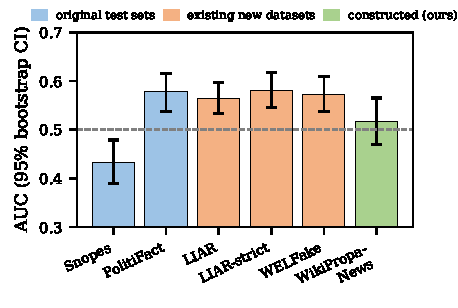
\includegraphics[width=\columnwidth]{fig_auc.pdf}
\caption{AUC with 95\% bootstrap CIs; the dashed line marks chance.}
\label{fig:auc}
\end{figure}

On new existing data, the detector transfers about as well as it does to the paper's own PolitiFact test set. LIAR, LIAR-strict and WELFake reach AUCs of 0.56--0.58 with CIs that overlap PolitiFact's and lie entirely above chance. The original method's weak but genuine signal therefore carries over to unseen sources, at least for this checkpoint. WikiPropaNews is the only new test set on which the detector does not beat chance.

\subsection{LIAR: Correct Ranking, Unusable Threshold}

On LIAR the detector predicts real for 99.9--100\% of statements. Its repository-style F1 of 0.72 is an artefact of always predicting the majority class; macro-F1 of 0.31--0.36 shows that the 0.5 threshold is useless here. Its AUC is nonetheless above chance, so the ranking carries signal even though the threshold does not. The likely cause is input length: LIAR statements average 18 words, against about 1,200 for PropaNews training articles. Dropping the ambiguous half-true class raises AUC slightly, from 0.564 to 0.581.

\subsection{WikiPropaNews by Fake Type and Topic}

The detector cannot distinguish WikiPropaNews fakes from real articles (CI includes 0.5), and no fake type differs reliably from chance (Table~\ref{tab:paired}). The task is deliberately hard: about 87\% of each fake is genuine, well-written journalism. A second factor is temporal. The paper itself reports that RoBERTa's accuracy on PolitiFact fakes falls from 69.0\% for articles before 2019 to 51.9\% for those after, and every WikiPropaNews article dates from 2020 or later. Topic makes no difference (Table~\ref{tab:topic}): per-topic AUCs range from 0.48 to 0.54, so the political skew of the loaded-language fakes does not drive the result.

\begin{table}[t]
\centering\small
\setlength{\tabcolsep}{4pt}
\begin{tabular}{lrr|lrr}
\toprule
Topic & $n$ & AUC & Topic & $n$ & AUC \\
\midrule
Politics & 200 & .528 & Sports & 38 & .478 \\
Crime/law & 78 & .519 & Health & 24 & .528 \\
Other & 76 & .538 & Sci./tech. & 24 & .476 \\
Disasters & 68 & .522 & Economy & 22 & .508 \\
Culture & 46 & .505 & & & \\
\bottomrule
\end{tabular}
\caption{WikiPropaNews AUC by topic (topics with at least 20 articles).}
\label{tab:topic}
\end{table}

\begin{table}[t]
\centering\small
\setlength{\tabcolsep}{3pt}
\begin{tabular}{lcrrrr}
\toprule
Fake type & AUC vs.\ real & \multicolumn{3}{c}{pairs: $+$\,/\,$-$\,/\,tie} & sign $p$ \\
\midrule
sent-fake & 0.504 & 40 & 45 & 15 & 0.66 \\
loaded-lang. & 0.511 & 63 & 32 & 2 & 0.002 \\
appeal-auth. & 0.536 & 65 & 31 & 4 & $<$0.001 \\
\bottomrule
\end{tabular}
\caption{By fake type: AUC of each type's fakes against all 297 real articles (all CIs include 0.5), and the within-pair test. A pair counts as ``$+$'' when the real article scores higher $P(\text{real})$ than its own fake; the two-sided sign test excludes ties.}
\label{tab:paired}
\end{table}

\subsection{Within-Pair Analysis}

Pooled AUC mixes two sources of variation: differences between articles and the effect of the edit. Figure~\ref{fig:hist} shows that the scores cluster by article, near 0.5 or near 0.1, while real and fake versions of the same article overlap almost completely. Comparing each fake with its own original removes the between-article variation.

When propaganda was inserted, the detector lowered $P(\text{real})$ in about two-thirds of pairs: 65 of 96 for appeal to authority ($p<0.001$) and 63 of 95 for loaded language ($p=0.002$). Both remain significant after a Bonferroni correction for three tests. When only a false claim was inserted, the detector did no better than chance (40 of 85, $p=0.66$). The shifts are tiny, with mean differences of 0.015 and 0.002, far too small to act on at any threshold.

Even so, this is direct evidence about the paper's mechanism. The PropaNews-trained detector has learned to respond to propagandistic style, not to falsity. This agrees with the paper's ablation, in which removing propaganda from training lowers transfer, and it explains why minimally falsified articles evade the detector.

\begin{figure}[t]
\centering
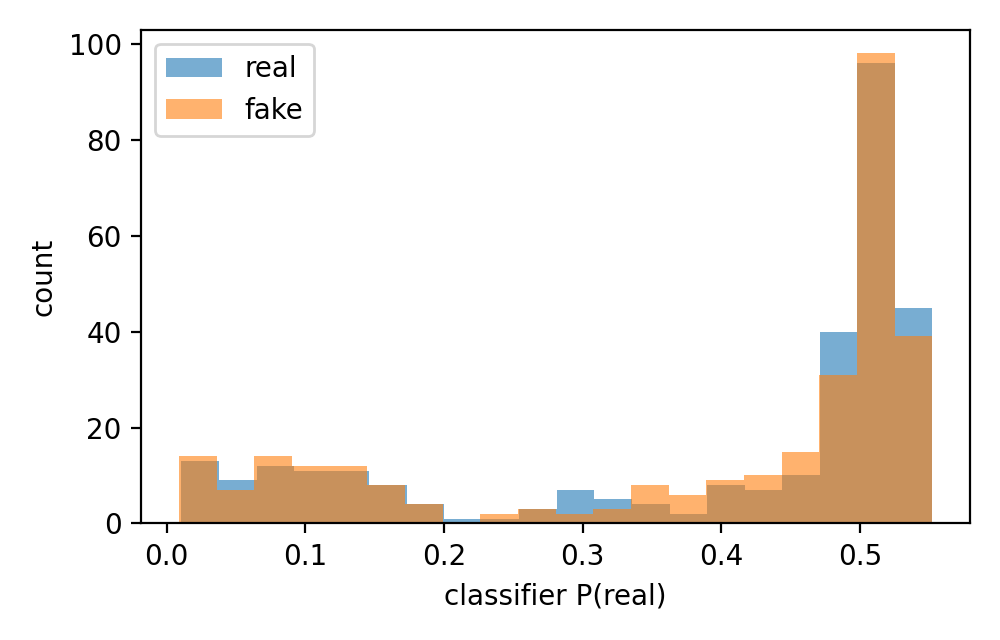
\includegraphics[width=0.95\columnwidth]{fig_prob_hist_wikipropanews.png}
\caption{Detector scores on WikiPropaNews. Real and fake versions overlap almost completely, and no score exceeds 0.55, consistent with the under-trained checkpoint (Section~\ref{sec:replication}).}
\label{fig:hist}
\end{figure}

\subsection{How the LLM-as-Judge Fitted into the Evaluation}

The judge validates the data, not the detector. It confirms at scale that each fake contains the intended falsehood and technique, which lets us interpret the per-type results as effects of those techniques rather than of generation noise. Its plausibility ratings add a further observation: appeal-to-authority fakes look most credible to a reader, and they also produced the largest within-pair shift in the detector. The detector is thus most sensitive to the technique that makes a fake most believable. Comparing the judge with the human annotator (Section~\ref{sec:human}) shows where its labels can be trusted: agreement is reasonable for contradiction and authority, but not for loaded language.

\section{Ethical Considerations}
\label{sec:ethics}

\subsection{Ethical Issues in the Original Paper}

The authors acknowledge that their generator is dual-use: it could produce realistic disinformation and toxic text. They therefore released the detectors and data but not the generator. Their crowdworkers were paid USD 12--15 per hour, and the paper carries a content warning. Their appeal-to-authority step, however, attributes fabricated quotations to real people drawn from Wikidata, and PropaNews, which contains these quotations, is publicly released.

\subsection{Ethical Issues in Publishing on Our New Data}

We assess our own work against the principles of the Australian Code for the Responsible Conduct of Research \citep{australiancode2018}.

\paragraph{Honesty and transparency.} We report negative and partial results, including the failed replication of effect sizes, the chance-level result on WikiPropaNews and the weak human agreement. We also document the correction of our earlier LIAR labels and the second annotation pass, rather than presenting only cleaned results.

\paragraph{Respect for persons and avoiding harm.} WikiPropaNews contains deliberately false statements, some about real public figures. For example, one fake edit makes a presidential spokesperson call his own leader ``reckless''. We mitigate this risk in four ways. We attribute every generated quotation to an unnamed authority, departing deliberately from PropaNews. Every fake is labelled and stored together with its original and source URL. We use only an off-the-shelf model with published prompts, so no new generation capability is released. Finally, our dataset card restricts the data to research on detection and warns against republishing individual fakes.

\paragraph{Fairness and recognition.} Wikinews text is used under CC BY 2.5 with attribution and a source link for every article. For LIAR and WELFake, our repository provides download-and-convert scripts instead of redistributing the third-party data. Likewise, we do not copy the authors' code, which carries no licence; a setup script fetches it from its source and applies our patch.

\paragraph{Human participants.} The only annotator was the author, so no participant data were collected. Scaling the annotation up to crowdworkers would require ethics approval, informed consent and fair pay, as in the original study.

\paragraph{Open access and accountability.} The project was possible only because the authors released their code and data. The dead checkpoint link nonetheless shows how quickly reproducibility decays when artefacts sit on personal cloud storage. We release all code, prompts, generated data, predictions and seeds, and recommend depositing them in an archive with a DOI.

\paragraph{AI assistance.} Generative AI (Claude) helped draft code and edit prose. The author ran every experiment, checked all outputs and is responsible for the content. All compute used was modest: about 3--4 GPU-hours on a T4.

\section{Conclusions and Reflections}
\label{sec:conclusion}

\paragraph{RQ1: Replication.} The released code runs after one small fix and transfers meaningfully above chance to PolitiFact, but we did not reproduce the reported AUCs (57.8 vs.\ 65.3 on PolitiFact and 43.3 vs.\ 53.0 on Snopes). The per-epoch log attributes the gap to training collapse at the learning-rate peak, compounded by an under-trained checkpoint, a single seed and two code--paper discrepancies.

\paragraph{RQ2: Existing datasets.} The replicated detector generalises to LIAR and WELFake as well as it does to the paper's own PolitiFact test set (AUC 0.56--0.58, all above chance). On short LIAR statements, however, its decision threshold is unusable.

\paragraph{RQ3: New data.} The detector fails on minimally falsified recent articles (AUC 0.52). The within-pair analysis nonetheless gives partial support for the paper's thesis: the detector does respond to propaganda techniques, but it does not respond to falsehood itself.

\paragraph{Reflections.} Three lessons stand out. First, asking an LLM to falsify and to add propaganda in a single prompt sacrifices the falsification: only 29\% of loaded-language edits contradicted the original. The paper's two-stage design, which generates the false claim before adding propaganda, is the better construction, and we would adopt it in future work. Second, annotation was unexpectedly difficult. Judging loaded language from long sentence pairs in a spreadsheet produced below-chance agreement, so a purpose-built interface and a second annotator would be needed for reliable human validation. Third, conventions must be verified, not assumed: label semantics differed from our expectations in both the original repository and WELFake, and one silent inversion had already distorted an earlier result.

\paragraph{Future work.} Future work should average several seeds, adjust the warm-up and the head learning rate, and use the authors' checkpoint if it becomes available again. It should also add a zero-shot LLM detector as a baseline on WikiPropaNews.

\bibliography{references}

\appendix

\section{Generation and Judge Prompts}
\label{app:prompts}

\paragraph{System prompt (all types).} ``You are assisting a university research project that builds a labelled test set for evaluating fake-news DETECTORS. The edited text is never published; it is stored with a FAKE label.'' The user prompt contains the article title, its first 250 words, the TARGET SENTENCE and one of the following tasks.

\paragraph{Sent-fake.} ``Rewrite the TARGET SENTENCE so that it states a specific, plausible but FALSE claim that contradicts the original (for example change a number, an outcome, who did what, where, or why). Keep a neutral, factual news style and roughly the same length. Do not add opinions or emotional words. Output ONLY the rewritten sentence.''

\paragraph{Loaded-language.} As above, but adding ``and write it using LOADED LANGUAGE: emotionally charged words meant to provoke a reaction (e.g.\ `shocking', `reckless', `devastating', `slammed')''.

\paragraph{Appeal-to-authority.} ``Line 1: rewrite the TARGET SENTENCE so that it states a specific, plausible but FALSE claim that contradicts the original, in a neutral factual news style. Line 2: write ONE new sentence containing a direct quotation that supports the false claim, attributed to a credible-sounding but UNNAMED authority relevant to the story \ldots\ Never name a real person as the source of the quote.''

\paragraph{Judge.} The judge sees the ORIGINAL SENTENCE and the EDITED PASSAGE and answers four questions. (1) Contradicts: does the edited passage make a claim inconsistent with the original? (2) Loaded language: does it use emotionally charged wording beyond neutral news style? (3) Appeal to authority: does it cite an authority to lend credibility, where the original does not? (4) Plausible: how believable is it as real news, from 1 (obviously fake) to 3 (fully plausible)? It returns a JSON object.

\section{Full Training Log}
\label{app:log}

\begin{table}[h]
\centering\small
\begin{tabular}{rrrrl}
\toprule
Epoch & Train loss & Dev AUC & Dev F1 & \\
\midrule
1 & 464.92 & 0.541 & 0.139 & saved \\
2 & 453.71 & 0.591 & 0.607 & saved \\
3 & 444.92 & 0.655 & 0.480 & final \\
4 & 452.72 & 0.580 & 0.649 & \\
5 & 444.02 & 0.528 & 0.617 & \\
6 & 452.37 & 0.449 & 0.000 & \\
7 & 444.73 & 0.500 & 0.649 & \\
8 & 448.47 & 0.498 & 0.649 & \\
9 & 439.18 & 0.500 & 0.649 & \\
10 & 436.34 & 0.500 & 0.649 & \\
\bottomrule
\end{tabular}
\caption{Per-epoch log of the replication run. Epochs are 1-indexed; the raw log counts from 0. Each epoch is 628 steps and takes about 7.3 minutes.}
\end{table}

\section{Reproducing This Work}
\label{app:repro}

The repository is organised in four parts:
(i) a setup script that clones the authors' code at a pinned commit and applies the AdamW patch;
(ii) a new-data directory with numbered scripts that collect Wikinews articles, generate fakes, apply the NLI filter and build the dataset, run the LLM judge, compute annotation agreement and produce the analysis, together with scripts that prepare LIAR and WELFake and evaluate any JSON-lines file;
(iii) analysis scripts for the per-type NLI rates and the paired sign test;
(iv) a single Colab notebook that runs the whole pipeline in order.

Every long-running step appends to its output and resumes after interruption, and all sampling uses seed 42. The final WikiPropaNews files, judge outputs, annotation sheet, prediction files and the training log are included.

\end{document}
